\documentclass[letter]{article}
\renewcommand{\baselinestretch}{1.25}

\usepackage[margin=1in]{geometry}
\usepackage{physics}
\usepackage{amsmath}
\usepackage{graphicx}
\usepackage{hyperref}


% MATLAB Formating Code
\usepackage[numbered,framed]{matlab-prettifier}
\lstset{style=Matlab-editor,columns=fullflexible}
\renewcommand{\lstlistingname}{Script}
\newcommand{\scriptname}{\lstlistingname}

\allowdisplaybreaks

%opening
\title{MECH 6313 - Homework 1}
\author{Jonas Wagner}
\date{2021, February 1}

\begin{document}

\maketitle


\section{Problem 1 - Duffing's Equation}
Duffings Equation is exhibits chaotic behavior with certain parameters. It is discribed by the following:
\begin{displaymath}
	\ddot{y} + \delta \dot{y} - y + y^3 = \alpha \cos(\omega_t t)
\end{displaymath}

\textbf{Problem:}
Simulate the equation for $\delta = 0.05, \alpha = 0.4$, and $\omega_t = 1.3$.\\

\textbf{Solution:}
In matlab the nlsys class (something I have been developing to help in nonlin system simulation - \href{https://github.com/jonaswagner2826/MECH6313}{https://github.com/jonaswagner2826/MECH6313}) was used to simulate the system and plot the following phase plots and time responses. The MATLAB code for this assignment is available in \appendixname \ref{script:HW1}\\



\begin{figure}[h]
	\centering
	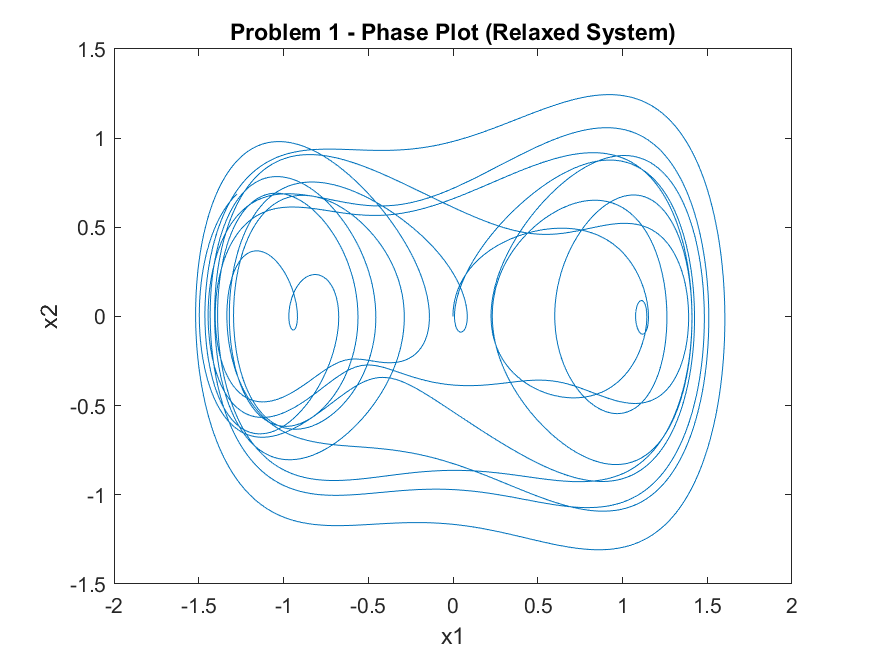
\includegraphics[width=0.7\linewidth]{fig/pblm1_phase}
	\caption{Phase Plot for the Relaxed System}
	\label{fig:pblm1phase}
\end{figure}


\begin{figure}[p]
	\centering
	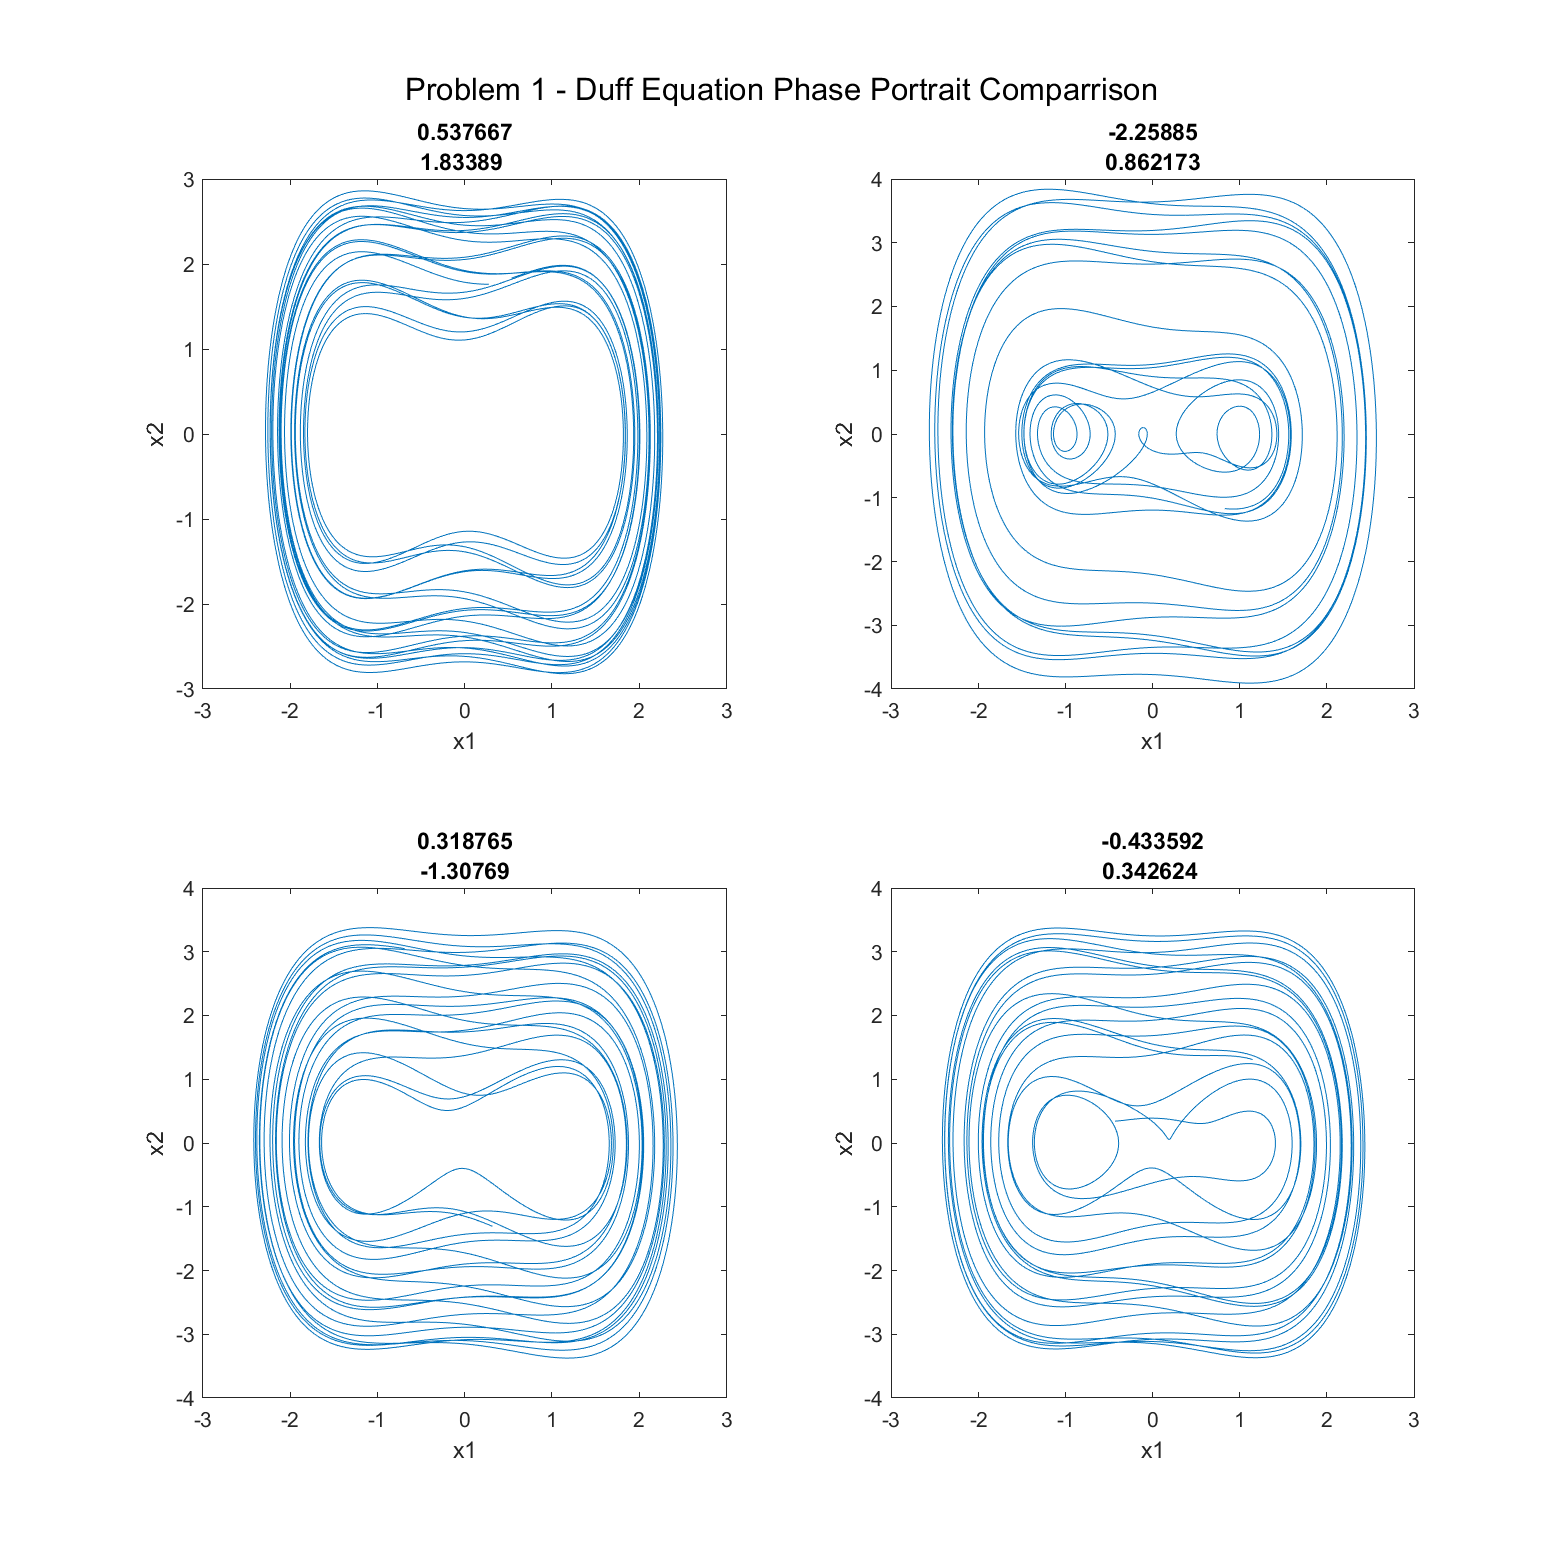
\includegraphics[width=1\linewidth]{fig/pblm1_phase_comparrision}
	\caption{Phase Plot for multiple initial conditions}
	\label{fig:pblm1phasecomparrision}
\end{figure}

\newpage
\begin{figure}[t]
	\centering
	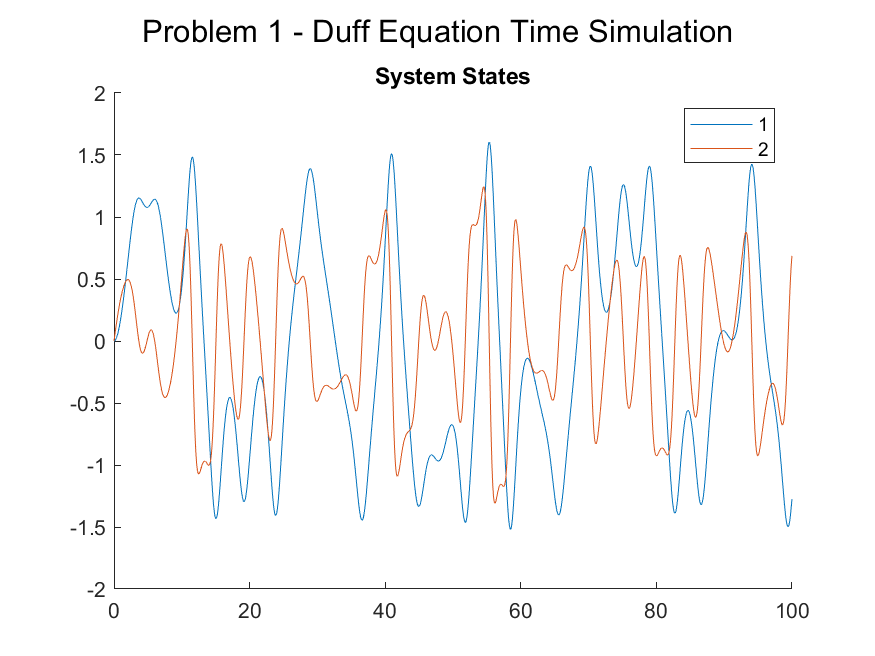
\includegraphics[width=0.8\linewidth]{fig/pblm1_vs_time}
	\caption{Plot of the relaxed system vs time}
	\label{fig:pblm1vstime}
\end{figure}


\textbf{Discussion:}\\








\newpage
\section{Problem 2 - Van Der Pol Equations}
\textbf{Problem:}
The van der Pole equation is as follows:
\begin{displaymath}
	\ddot{y} + \qty(y^2 - 1)*\dot{y} + y = 0
\end{displaymath}

Plot the phase portrait, time dependence and compare with the response of Duffing's equations.\\

\textbf{Solution:}







\begin{figure}[h]
	\centering
	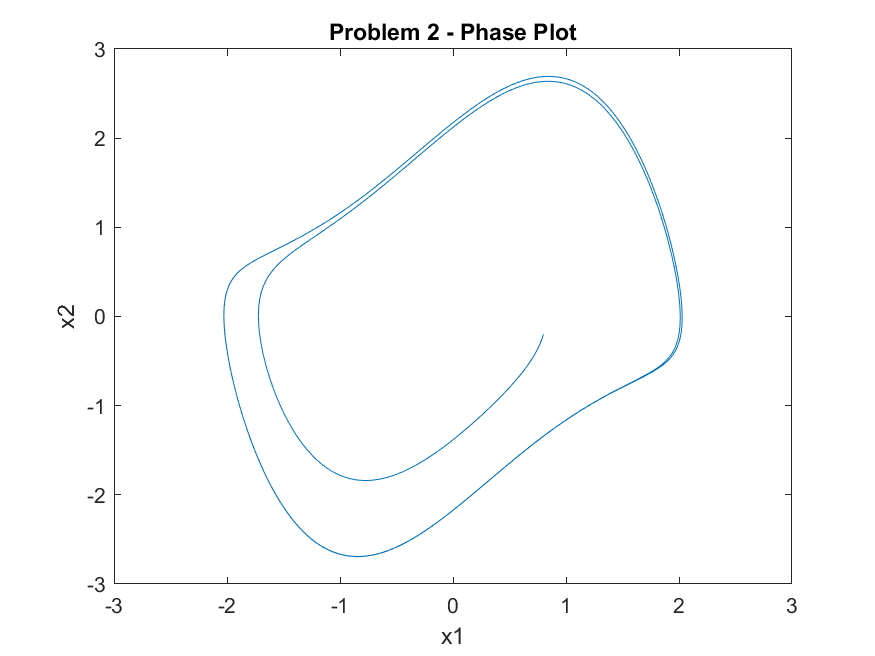
\includegraphics[width=0.7\linewidth]{fig/pblm2_phase}
	\caption{Phase Plot for the Relaxed System}
	\label{fig:pblm2phase}
\end{figure}


\begin{figure}[p]
	\centering
	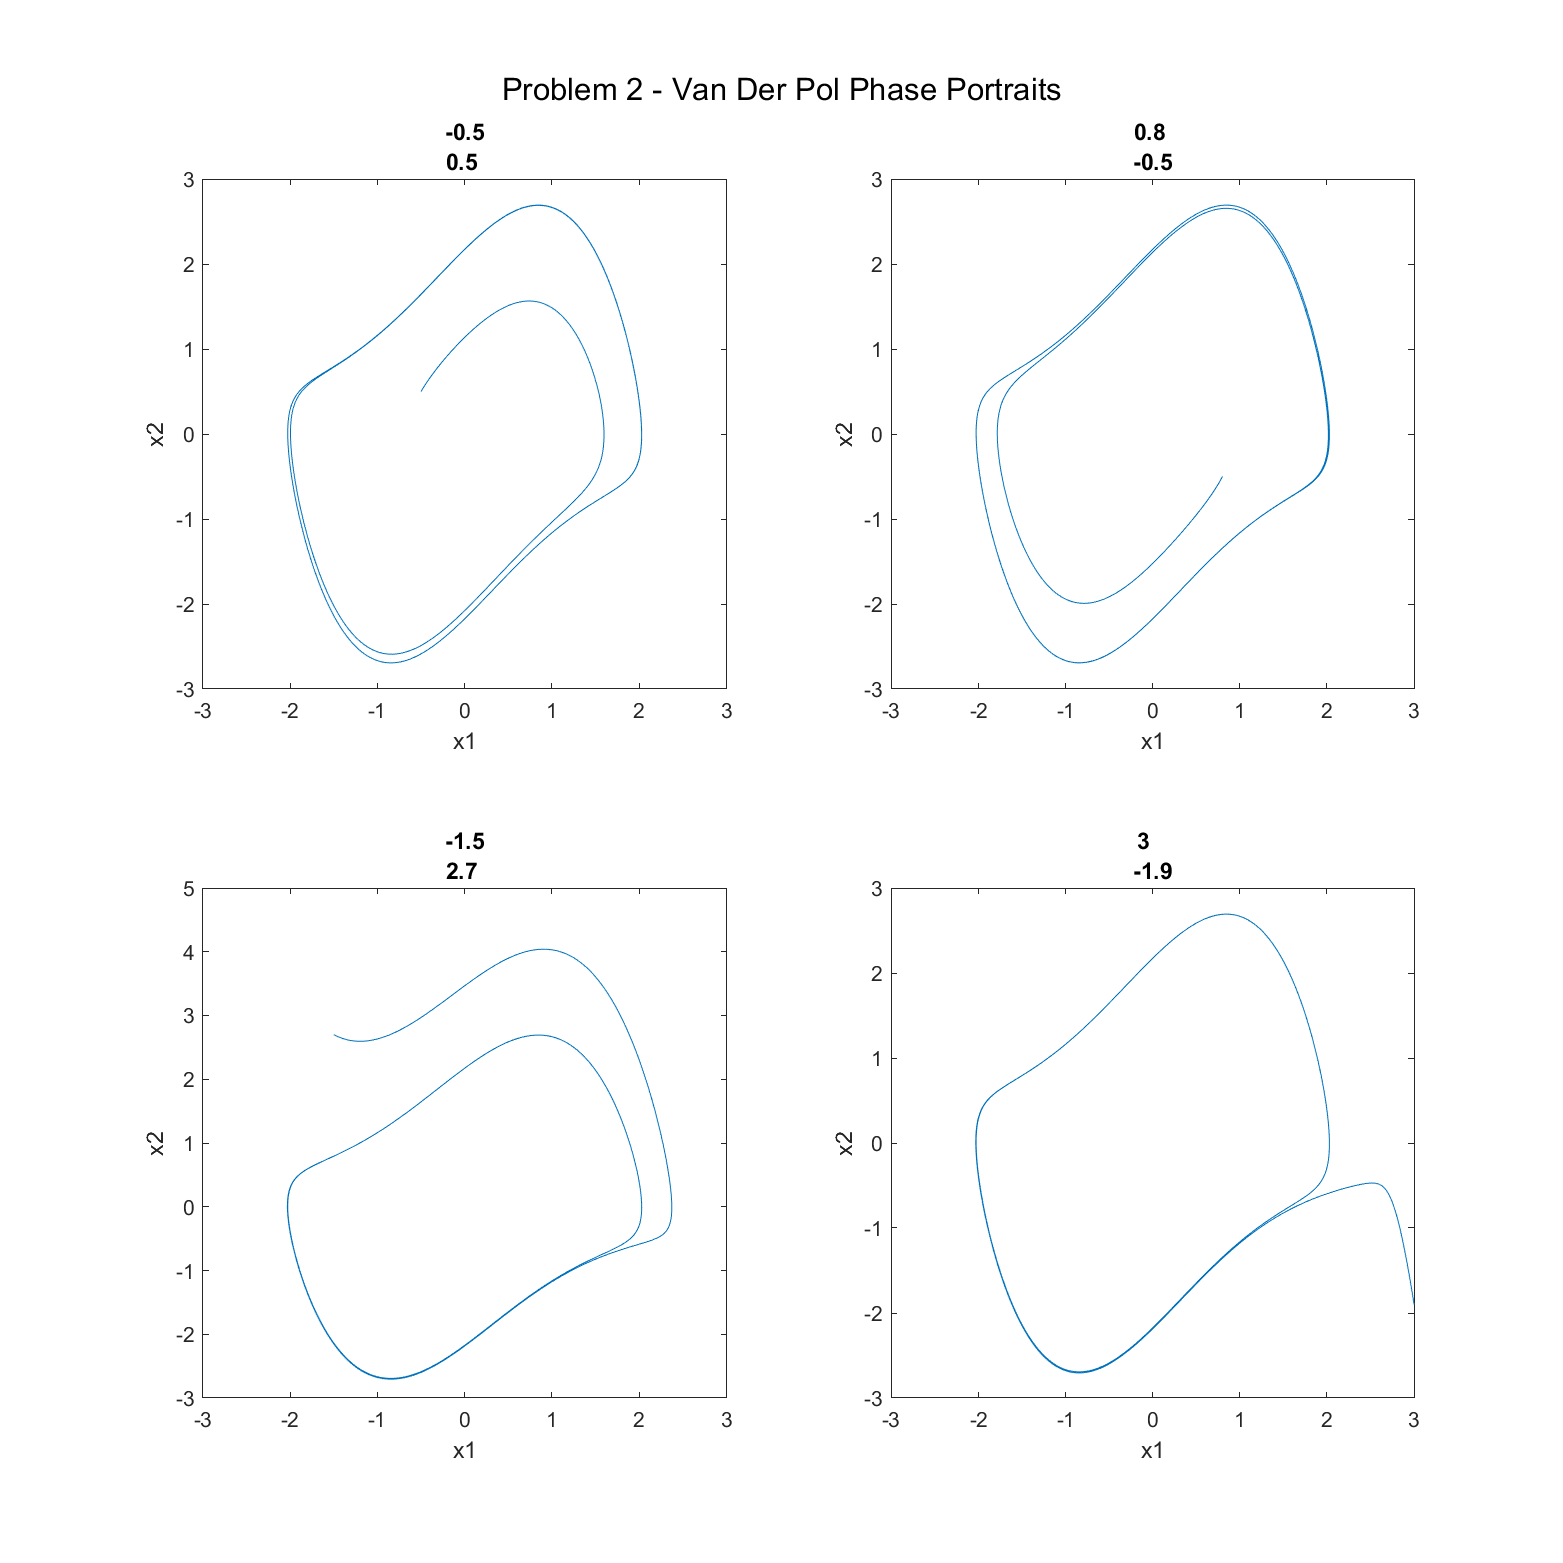
\includegraphics[width=1\linewidth]{fig/pblm2_phase_comparrision}
	\caption{Phase Plot for multiple initial conditions}
	\label{fig:pblm2phasecomparrision}
\end{figure}

\newpage
\begin{figure}[t]
	\centering
	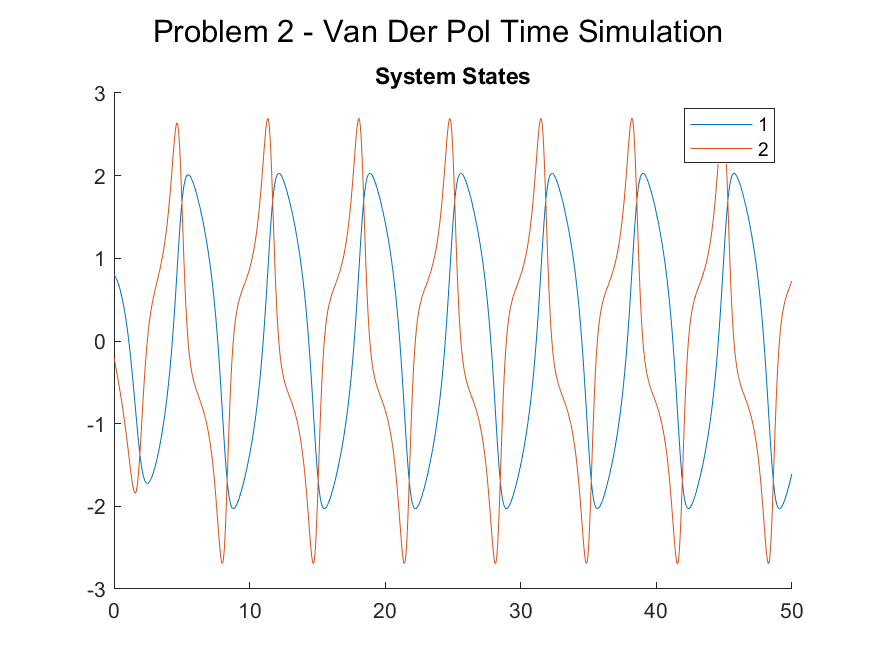
\includegraphics[width=0.8\linewidth]{fig/pblm2_vs_time}
	\caption{Phase Plot for multiple initial conditions}
	\label{fig:pblm2vstime}
\end{figure}


\textbf{Discussion:}


\newpage
\subsection{Negative Nonlinear Term}



\newpage
\appendix
\section{MATLAB Code:}
% MECH6313_HW1
\lstinputlisting[caption={MECH6313\_HW1},label={script:HW1}]{MECH6313_HW1.m}


\end{document}
